% Document properties
\documentclass[a4paper, finnish, 12pt, twoside]{article}
\usepackage[utf8]{inputenc}
\usepackage[T1]{fontenc}
\usepackage[finnish]{babel}

% LaTeX Packages
% Sorted by name
\usepackage{amsmath}	% Equations
\usepackage{amsfonts}	% Just in case to ensure better symbol fonts
\usepackage{amssymb}	% Mathematical symbols, \mathbb{}
\usepackage{array}		% Arrays
\usepackage{bm}			% Bold vector symbols
\usepackage{cite}		% Source citations
\usepackage{emptypage} 	% Clears unwanted artifacts from empty pages
\usepackage{esint}		% Symbols for integrals over closed lines (kiertointegraali) \oint \oiint
\usepackage{fancyhdr} 	% For custom header style
\usepackage{gensymb}	% For degree sign
\usepackage{graphicx}	% For including pictures
\usepackage{hyperref}	% Hyperlinks
\usepackage{longtable}	% Tables that span multiple pages: \longtable, required by longtabu
\usepackage{multirow}	% Table cells spanning multiple rows: \multirow
\usepackage{pslatex}	% Makes the PDF output look better
\usepackage{tabu}		% Tables that span multiple pages and the page width: \longtabu
\usepackage{tabularx}	% Tables that span the whole page width: \tabularx
\usepackage{titletoc,tocloft} % For styling Table of Contents
\usepackage{titlesec}	% For styling \part headers
\usepackage{xifthen}	% Expanded if-else-logic for functions, \ifthenelse for example


% Define Table of Contents style
\setcounter{tocdepth}{2}
\setlength{\cftsubsecindent}{4.5em}
\dottedcontents{section}[3em]{}{1.3em}{.6em}

% Define \part header style
\titleclass{\part}{top} % Make \part like a chapter
\titleformat{\part}
[display]
{\centering\normalfont\huge\bfseries}
{\titlerule[3pt]\vspace{3pt}\titlerule[1pt]\vspace{3pt}\MakeUppercase{\partname} \thepart}
{0pt}
{\huge\MakeUppercase}
[\vspace{-0.5em}\rule{\textwidth}{2pt}]

% Define the amount of whitespace to come after \part
\titlespacing*{\part}{0pt}{0pt}{40pt}

% Custom command for fetching the part name to the header
\newcommand*\parttitle{}
\let\origpart\part
\renewcommand*{\part}[2][]{%
	\ifx\\#1\\% optional argument not present?
		\origpart{#2}%
		\renewcommand*\parttitle{#2}%
	\else
		\origpart[#1]{#2}%
		\renewcommand*\parttitle{#1}%
	\fi
}

% Preventing problems caused by the Unicode non-breaking space character
% Without this declaration the compiler would crash if the user has inserted such character by mistake
% Now it just generates an error text
\DeclareUnicodeCharacter{00A0}{UNICODE_ERROR}

%-----
% Environment and command definitions

% It's highly recommended to use these whenever possible so that the style of the whole document can be changed from here

% Basic table for physical constants
\newenvironment{consttable}[1]{
	\begin{table}[!ht]
	\centering
	\caption{#1}
	\setlength{\extrarowheight}{5pt}
	\begin{tabular}{|l| >{$\displaystyle} l <{$} | l |}
	\hline
}{
	\hline
	\end{tabular}
	\end{table}
}

% Basic table for label & equation
\newenvironment{eqtable}[1]{
	\begin{table}[!ht]
	\centering
	\caption{#1}
	\setlength{\extrarowheight}{10pt}
	\begin{tabular}{| l | >{$\displaystyle} l <{$} |}
	\hline
}{
	\hline
	\end{tabular}
	\end{table}
}

% Basic table with columns for symbol and units
\newenvironment{eqtable-units}[1]{
	\begin{table}[!ht]
	\centering
	\caption{#1}
	\setlength{\extrarowheight}{10pt}
	\begin{tabular}{| l | >{$} l <{$} | l | >{$\displaystyle} l <{$} |}
	\hline
}{
	\hline
	\end{tabular}
	\end{table}
}

% Basic table for math without labels
\newenvironment{mathtable}[1]{
	\begin{table}[!ht]
	\centering
	\caption{#1}
	\setlength{\extrarowheight}{10pt}
	\begin{tabular}{| >{$\displaystyle} l <{$} |}
	\hline
}{
	\hline
	\end{tabular}
	\end{table}
}

% Matrix with style that can be changed from here
\newenvironment{styledmatrix}{
	\setlength{\extrarowheight}{0pt}
	\begin{bmatrix}
}{
	\end{bmatrix}
}

% Systems of multiple equations (yhtälöryhmä)
\newenvironment{eqgroup}{
	\setlength{\extrarowheight}{0pt}
	\begin{cases}
}{
	\end{cases}
}

% Inner product
\newcommand{\innerp}[2]{
	\langle \bm{#1}, \bm{#2} \rangle
}

% Laplace transform
\newcommand{\laplace}[1]{
	\ifthenelse{\isempty{#1}}{
		\mathcal{L}
	}{
		\mathcal{L} \{ #1 \}
	}
}

%-----

% Document metadata
\title{Linnunradan käsikirja teekkareille}
\author{Tampereen teekkarit}
\date{\the\day.\the\month.\the\year}


\begin{document}

% Title page
\begin{titlepage}
\centering
{\huge Linnunradan käsikirja teekkareille \par}
% {\large Tampereen teekkarit \par}
{\the\day.\the\month.\the\year \par}
\vfill
\includegraphics{by-sa.eps}
\end{titlepage}

\pagenumbering{roman} % Start with roman numbers

% Foreword
Maailma on kaavoja ja taulukoita täynnä, mutta ne ovat olleet hajallaan useissa kirjoissa,
joista tiedon etsiminen on hidasta - varsinkin paperiversioista, joissa Ctrl+F ei luonnollisesti toimi.
Lisäksi monet niistä ovat tiukkojen tekijänoikeuksien ja kopiokieltojen alaisia,
vaikka tieto itsessään on vapaata. Nyt niille on vaihtoehto. Ole hyvä.

% Disclaimer
Tämä kirja on opiskelijaprojekti, joten emme voi ottaa vastuuta mahdollisista virheistä.
Toivommekin, että ilmoitat niistä vaikkapa \href{https://github.com/AgenttiX/compendium}{GitHubin} kautta, jotta voimme korjata ne.

% Credits
\begin{table*}[h!]
\centering
\begin{tabular}{ll}
Mika \textit{AgenttiX} Mäki		& Projektin perustaja \\
Daniel \textit{Ohems} Saarimäki \\
% Add name here					% Add title here
\end{tabular}
\end{table*}

% License
\vfill
{
	\centering
	\href{https://creativecommons.org/licenses/by-sa/4.0/}{Creative Commons Attribution-ShareAlike 4.0 International}
	\par
}

% Table of Contents
\pagebreak
\tableofcontents
\vfill % Prevents TOC from expanding to full page height

% Define header
\pagestyle{fancy}
\fancyhead{} 
\fancyhead[LO,RE]{\MakeUppercase{\textit{\parttitle}}} 
\fancyhead[RO,LE]{\nouppercase{\textit{\rightmark}}}
\fancyfoot{}
\fancyfoot[C]{\thepage}

% Main content
\pagebreak
\pagenumbering{arabic} % Switch back to arabic page numbers



\part{Matematiikka}

\chapter{Merkintöjä}

%-----
\iffalse
\chapter{Alkulukuja}
% https://www.cs.cmu.edu/~dst/DeCSS/Gallery/Stego/illegal-primes.html
4856507896573978293098418946942861377074420873513579240196520736 \\
6869851340104723744696879743992611751097377770102744752804905883 \\
1384037549709987909653955227011712157025974666993240226834596619 \\
6060348517424977358468518855674570257125474999648219418465571008 \\
4119086259716947970799152004866709975923596061320725973797993618 \\
8606316914473588300245336972781813914797955513399949394882899846 \\
9178361001825978901031601961835034344895687053845208538045842415 \\
6548248893338047475871128339598968522325446084089711197712769412 \\
0795862440547161321005006459820176961771809478113622002723448272 \\
2493232595472346880029277764979061481298404283457201463489685471 \\
6908235473783566197218622496943162271666393905543024156473292485 \\
5248991225739466548627140482117138124388217717602984125524464744 \\
5055834628144883356319027253195904392838737640739168912579240550 \\
1562088978716337599910788708490815909754801928576845198859630532 \\
3823490558092032999603234471140776019847163531161713078576084862 \\
2363702835701049612595681846785965333100770179916146744725492728 \\
3348691600064758591746278121269007351830924153010630289329566584 \\
3662000800476778967984382090797619859493646309380586336721469695 \\
9750279687712057249966669805614533820741203159337703099491527469 \\
1835659376210222006812679827344576093802030447912277498091795593 \\
8387121000588766689258448700470772552497060444652127130404321182 \\
610103591186476662963858495087448497373476861420880529443 \\
Huomioithan, että tämän sivun hallussapito on laitonta Yhdysvalloissa.
\fi
%-----

\chapter{Differentiaali- ja integraalilaskenta}

\section{Derivointi}

\section{Integrointi}


\chapter{Vektorit ja matriisit \cite{MAT-60000}}

\section{Vektorit}

\begin{taulukko}{Vektorien perusteet}
Vektori						& \bm{x} = \begin{matriisi} x_1 \\ x_2 \\ \vdots \\ x_n \end{matriisi} \\ \hline
Luonnolliset kantavektorit	& \bm{e}_i = \begin{matriisi} 0 \\ \vdots \\ 0 \\ 1 \\ 0 \\ \vdots \\ 0 \end{matriisi}, \qquad i \in \mathbb{Z}^+ \\ \hline
Nollavektori				& \bm{0} = \begin{matriisi} 0 \\ \vdots \\ 0 \end{matriisi} \\ \hline
Vektorien summa				& \bm{x} + \bm{y} = \begin{matriisi} x_1 \\ x_2 \\ \vdots \\ x_n \end{matriisi} + 
							\begin{matriisi} y_1 \\ y_2 \\ \vdots \\ y_n \end{matriisi} =
                            \begin{matriisi} x_1 + y_1 \\ x_2 + y_2 \\ \vdots \\ x_n + y_n \end{matriisi}
                            \\ \hline
Vektorien erotus			& \bm{x} - \bm{y} = \bm{x} + (-\bm{y}) \\ \hline
\end{taulukko}

Vektoriavaruuksien aksioomat
\begin{align*}
(1)	\quad & \bm{x} + \bm{y} = \bm{y} + \bm{x} \\
(2)	\quad & (\bm{x} + \bm{y}) + \bm{z} = \bm{x} + (\bm{y} + \bm{z}) \\
(3)	\quad & \bm{x} + \bm{0} = \bm{0} + \bm{x} = \bm{x} \\
(4) \quad & \bm{x} + (-\bm{x}) = (-\bm{x}) + \bm{x} = \bm{0} \\
(5) \quad & \alpha ( \bm{x} + \bm{y} ) = \alpha \bm{x} + \alpha \bm{y} \\
(6) \quad & (\alpha + \beta ) \bm{x} = \alpha \bm{x} + \beta \bm{x} \\
(7) \quad & \alpha ( \beta \bm{x} ) = (\alpha \beta) \bm{x} \\
(8) \quad & 1 \bm{x} = \bm{x}
\end{align*}

\begin{taulukko}{Sisätulo ja normi}
Sisätulo					& \sisatulo{x}{y} = \sum^n_{i=1} \overline{x_i} y_i = \bm{x}^* \bm{y} \\ \hline
Sisätulon perusominaisuudet	& (1) \quad \sisatulo{x}{y} \geq 0 \land (\sisatulo{x}{y} = 0 \rightarrow \bm{x} = \bm{0}) \\
							& (2) \quad \langle \bm{x} + \bm{y}, \bm{z} \rangle = \sisatulo{x}{z} + \sisatulo{y}{z} \\
                           	& (3) \quad \langle \bm{x}, \alpha \bm{y} \rangle = \alpha \sisatulo{x}{y} \\
                            & (4) \quad \sisatulo{x}{y} = \overline{\sisatulo{y}{x}} \\
                            & \forall \bm{x}, \bm{y}, \bm{z} \in \mathbb{C}^n, \alpha \in \mathbb{C} \\ \hline
Ortogonaalisuus				& \sisatulo{x}{y} = 0 \\ \hline
Kroneckerin symboli			& \delta_{ij} \begin{yhtaloryhma} 0 \quad i \neq j \\ 1 \quad i=j \end{yhtaloryhma} \\ \hline
Vektorijoukon ortogonaalisuus	& \langle \bm{x}_i, \bm{x}_j \rangle \begin{yhtaloryhma} 0 \quad i \neq j \\ \neq 0 \quad i=j \end{yhtaloryhma} \\
Vektorijoukon ortonormaalius	& \langle \bm{x}_i, \bm{x}_j \rangle = \delta_{ij} \\ \hline
Normi						& ||\bm{x}|| = \sqrt{\sisatulo{x}{x}} \\ \hline
Normin ominaisuudet			& (1) \quad || \bm{x} || \geq 0 \land (|| \bm{x} || = 0 \leftrightarrow \bm{x} = \bm{0}) \\
							& (2) \quad || \alpha \bm{x} || = | \alpha | || \bm{x} || \quad \forall \alpha \in \mathbb{C}^n \\
Kolmioepäyhtälö				& (3) \quad || \bm{x} + \bm{y} || \leq || \bm{x} || + || \bm{y} || \\ \hline
Kolmioepäyhtälö alaspäin	& || \bm{x} - \bm{y} || \geq \big| || \bm{x} || - || \bm{y} || \big| \\ \hline
Cauchy-Schwarzin epäyhtälö	& |\sisatulo{x}{y}| \leq || \bm{x} || \cdot || \bm{y} || \\ \hline
Vektorien välinen kulma		& \cos(\phi) = \frac{\sisatulo{x}{y}}{|| \bm{x} || \cdot || \bm{y} ||} \\ \hline
\end{taulukko}


\section{Matriisit}

\begin{taulukko}{Matriisien perusteet}
Lineaarikuvaus				& L(a \bm{x} + b \bm{y}) = a L(\bm{x}) + b L({\bm{y})} \\ \hline
Matriisin indeksointi		& A=[a_{ij}]^{m\times n} = 
                			\begin{matriisi} a_{11}  & a_{12}  & \dots  & a_{1n} \\ 
							a_{21}  & a_{22}  & \dots  & a_{2n} \\ 
							\vdots  & \vdots & \ddots & \vdots \\ 
							a_{m1}  & a_{m2}  & \dots  & a_{mn} \end{matriisi} \\
                            
							& \text{m on korkeus (vaakarivien määrä)} \\
                           	& \text{n on leveys (pystyrivien määrä)} \\ \hline

Neliömatriisi				& m=n \\
Korkea matriisi				& m>n \\
Leveä matriisi				& m<n \\ \hline
Sarakevektorit				& A = \begin{matriisi} \bm{a}_1, \bm{a}_2, \ldots, \bm{a}_n\end{matriisi} \\
Vaakarivivektorit			& A = \begin{matriisi} \bm{a}^T_1 \\ \bm{a}^T_2 \\ \vdots \\ \bm{a}^T_m \end{matriisi} \\ \hline
Neliömatriisin jälki		& \text{tr}(A) = \sum^n_{i=1} a_{ii} \text{ eli diagonaalialkioiden summa} \\ \hline
Matriisien summa			& A + B = (a_{ij}) + (b_{ij}) = (a_{ij} + b_{ij}) \\
Skalaarilla kertominen		& \alpha A = (\alpha a_{ij}) \\
Matriisien erotus			& A - B = A + (-1)B = (a_{ij}) + (-b_{ij}) = (a_{ij} - b_{ij}) \\ \hline
Matriisien tulo				& C = (c_{ij})_{m \times n} = \big( \sum^p_{k=1} a_{ik} b_{kj} \big)_{m \times n} \\ \hline
Matriisien laskusäännöt		& (A+B)+C = A+(B+C) \\
							& (AB)C = A(BC) \\
                            & A(B+C) = AB + AC \\
                            & (A+B)C = AC + BC \\
                            & A + B = B + A \\ \hline
Neliömatriisin potenssit	& A^k = AA \cdots A \\ \hline
\end{taulukko}


\begin{taulukko}{Matriisityyppejä}
Identiteettimatriisi		& I = \begin{matriisi}
							\bm{e}_1, \bm{e}_2, \ldots, \bm{e}_n
							\end{matriisi} = 
							\begin{matriisi}
							1 & 0 & \cdots & 0 \\
                            0 & 1 & \cdots & 0 \\
                            \vdots & \vdots & \ddots & \vdots \\
                            0 & 0 & \cdots & 1 \\
							\end{matriisi} \\ \hline
Lohkomatriisi				& A =
							\begin{matriisi}
                            A_{11} & A_{12} & \cdots & A_{1q} \\
                            \vdots & & & \vdots \\
                            A_{p1} & A_{p2} & \cdots & A_{pq} \\
                            \end{matriisi} \\ \hline
                            
Diagonaalimatriisi			& A = \text{diag}(a_{11}, a_{22}, \ldots, a_{nn}) = 
							\begin{matriisi}
                            a_{11} & 0 & \cdots & 0 \\
                            0 & a_{22} & \cdots & 0 \\
                            \vdots & \vdots & \ddots & \vdots \\
                            0 & 0 & \cdots & a_{nn}
                            \end{matriisi} \\ \hline

Yläkolmiomatriisi			& (i>j \rightarrow a_{ij} = 0) \Leftrightarrow A =
							\begin{matriisi}
                            a_{11} & a_{12} & \cdots & a_{1n} \\
                            0 & a_{22} & \cdots & a_{2n} \\
                            \vdots & \vdots & \ddots & \vdots \\
                            0 & 0 & \cdots & a_{mn}
                            \end{matriisi}
							\\
Alakolmiomatriisi			& (i<j \rightarrow a_{ij} = 0) \Leftrightarrow A = 
							\begin{matriisi}
                            a_{11} & 0 & \cdots & 0 \\
                            a_{21} & a_{22} & \cdots & 0 \\
                            \vdots & \vdots & \ddots & \vdots \\
                            a_{m1} & a_{m2} & \cdots & a_{mn}
                            \end{matriisi}
                            \\ \hline
Lohkodiagonaalinen matriisi	& A = diag(A_{11}, A_{22}, \ldots, A_{pp})
							\begin{matriisi}
                            A_{11} & O & \cdots & O \\
                            O & A_{22} & \cdots & O \\
                            \vdots & \vdots & \ddots & \vdots \\
                            O & O & \cdots & A_{pp}
                            \end{matriisi} \\ \hline
Lohkoalakolmiomatriisi		& A = 
							\begin{matriisi}
                            A_{11} & A_{12} & \cdots & A_{1q} \\
                            O & A_{22} & \cdots & A_{2q} \\
                            \vdots & \vdots & \ddots & \vdots \\
                            O & O & \cdots & A_{pq}
                            \end{matriisi}
							\\
Lohkoyläkolmiomatriisi		& A =
							\begin{matriisi}
                            A_{11} & O & \cdots & O \\
                            A_{21} & A_{22} & \cdots & O \\
                            \vdots & \vdots & \ddots & \vdots \\
                            A_{p1} & A_{p2} & \cdots & A_{pq}
                            \end{matriisi}
							\\ \hline
Permutaatiomatriisi			& P = \begin{matriisi}
							\bm{e}^T_{r_1} \\ \bm{e}^T_{r_1} \\ \vdots \\ \bm{e}^T_{r_n}
                            \end{matriisi}
							= \text{esim.} \begin{matriisi} 0&0&1 \\ 0&1&0 \\ 1&0&0 									\end{matriisi} \\ \hline
\end{taulukko}


\begin{taulukko}{Transpoosi ja konjugaattitranspoosi}
Transpoosi					& A^T = (a_{ji})_{n \times m} =
							\begin{matriisi}
                            a_{11} & a_{21} & \cdots & a_{m1} \\
                            a_{12} & a_{22} & \cdots & a_{m2} \\
                            \vdots & \vdots & \ddots & \vdots \\
                            a_{1n} & a_{2n} & \cdots & a_{nm} \\
                            \end{matriisi} \\

Konjugaattitranspoosi       & A^* = (\overline{a}_{ji})_{m \times n} =
							\begin{matriisi}
                            \overline{a}_{11} & \overline{a}_{21} & \cdots & \overline{a}_{m1} \\
                            \overline{a}_{12} & \overline{a}_{22} & \cdots & \overline{a}_{m2} \\
                            \vdots & \vdots & \ddots & \vdots \\
                            \overline{a}_{1n} & \overline{a}_{2n} & \cdots & \overline{a}_{nm} \\
                            \end{matriisi}\\ \hline

Transpoosille				& (AB)^T = B^T A^T \\
							& (A+B)^T = A^T + B^T \\
                            & (\alpha A)^T = \alpha A^T \\ \hline

Konjugaattitranspoosille	& (AB)^* = B^* A^* \\
							& (A+B)^* = A^* + B^* \\
							& (\alpha A)^* = \overline{\alpha} A^* \\ \hline
\end{taulukko}


\begin{taulukko}{Matriisien ominaisuuksia}
Kommutoivuus				& AB = BA \\ \hline

Symmetrisyys				& A = A^T \\
Hermiittisyys				& A = A^* \\
Vinosymmetrisyys			& A = -A^T \\
Vinohermiittisyys			& A = -A^* \\ \hline

Singulaarisuus				& det(A) = 0 \\
Ei-singulaarisuus			& det(A) \neq 0 \\
							& \exists A^{-1} \\ \hline

Ortogonaalisuus				& A^T A = I = AA^T \\
Unitaarisuus				& U^* U = U U^* = I \\ \hline

Inverssi					& A A^{-1} = I = A^{-1} A \\
							& (AB)^{-1} = B^{-1} A^{-1} \\
                           	& (A^{-1})^{-1} = A \\ \hline
\end{taulukko}


\begin{taulukko}{Lineaarinen yhtälöryhmä}
Lineaarinen yhtälöryhmä		& A \bm{x} = \bm{b} \\
							& \bm{x} = A^{-1} \bm{b} \\ \hline
\end{taulukko}


\begin{taulukko}{Hermiittisille matriiseille}
Positiivisesti definiitti		& \langle \bm{x}, A \bm{x}\rangle > 0, \forall \bm{x} \neq \bm{0} \\
Positiivisesti semidefiniitti	& \langle \bm{x}, A \bm{x}\rangle \geq 0, \forall \bm{x} \\
Negatiivisesti definiitti		& \langle \bm{x}, A \bm{x}\rangle < 0, \forall \bm{x} \neq \bm{0} \\
Negatiivisesti semidefiniitti	& \langle \bm{x}, A \bm{x}\rangle \leq 0, \forall \bm{x} \\
Indefiniitti					& \text{Jos ei ole mitään näistä} \\ \hline
\end{taulukko}


\begin{taulukko}{LU-hajotelma}
LU-hajotelma	& A = LU \\
				& L_k = I - \bm{l}_k \bm{e}^T_k \\
                & \bm{l}_k = \frac{1}{x_k} \begin{matriisi} 0 \\ \vdots \\ 0 \\ x_{k+1} \\ \vdots \\ x_n \end{matriisi}, x_k \neq 0 \\
                & L_{n-1} L_{n-2} \cdots L_1 A = U \\
                & \hat{L} = L_{n-1} L_{n-2} \cdots L_1 \\
                & A = \hat{L}^{-1} U = LU \\ \hline
Jos ei onnistu suoraan, niin viimeistään	& PA = LU, \text{ jossa P on permutaatiomatriisi} \\ \hline
Lineaarisen yhtälöryhmän ratkaiseminen	& A \bm{x} = P^T LU \bm{x} = \bm{b} \\
											& LU \bm{x} = P \bm{b} \\
                                            & L \bm{y} = P \bm{b} \land U \bm{x} = \bm{y} \\
                                            & x = U^{-1} \bm{y} \land \bm{y} = L^{-1} P \bm{b} \\ \hline
\end{taulukko}


\begin{taulukko}{Aliavaruus}
Aliavaruus					& \alpha \bm{x} + \beta \bm{y} \in S \quad \forall \bm{x}, \bm{y} \in \mathcal{S} \\
Arvojoukko (kuva-avaruus)	& \mathcal{R} (A) = \{y | \exists \bm{x} \in \mathbb{F}^n s.e. \bm{y} = A \bm{x} \} \in \mathbb{F}^m \\
Ydin (nolla-avaruus)		& \mathcal{N} (A) = \{ \bm{x} | A \bm{x} = \bm{0} \} \\ \hline

Ortogonaalikomplementti		& \mathcal{S}^\perp = \{ \bm{y} | \langle \bm{y}, \bm{x} \rangle = 0, \forall \bm{x} \in \mathcal{S} \} \\ \hline

							& \mathcal{N} (A) = \mathcal{R} (A^*)^\perp \\
                            & \mathcal{N} (A^*) = \mathcal{R} (A)^\perp \\ \hline

Dimensio eli kantavektorien lukumäärä	& \dim (S) \\
Matriisin aste							& rank (A) = \dim \mathcal{R} (A) \\
										& rank (A) + \dim \mathcal{N} (A) = n = \text{ sarakkeiden määrä} \\ \hline

Projektorimatriisi			& P^2 = P \\
							& \text{Projisoi vektorit } \mathcal{R} (P) \text{:lle pitkin } \mathcal{N} (P) \text{:tä} \\ \hline
\end{taulukko}


\begin{taulukko}{Ominaisarvot ja -vektorit}
Ominaisarvot ja -vektorit	& A \bm{x} = \lambda \bm{x}, \bm{x} \neq \bm{0} \\
Ominaisarvot				& \det (A - \lambda I) = 0 \\
Karakteristinen polynomi	& \prod^n_{k=1} (\lambda - \lambda_k) \\
Spektri						& \sigma (A) = \{ \lambda_ 1, \lambda_2, \ldots , \lambda_n \} \\
Similaarisuus				& B = S^{-1} A S \text{ jossa S ei-singulaarinen}\\
Unitaarinen similaarisuus	& B = U^* AU \\

Hermiten matriisille		& diag(\sigma(A)) = U^* A U \\
							& \forall \lambda \in \mathbb{R} \land n \text{ ortonormaalia ominaisvektoria} \Rightarrow \text{Hermiten matriisi} \\ \hline

Normaali matriisi			& A = UDU^* \text{ jossa D on diagonaalimatriisi} \\ \hline
\end{taulukko}


\begin{taulukko}{Jordanin kanoninen muoto}
				& A = SJS^{-1} \\
				& J = diag(J_1, J_2, \ldots, J_p) \\
Defektiivisyys	& \exists \lambda : geom(\lambda) < alg(\lambda) \\ \hline
				& A \bm{s}^j_1 = \lambda_j \bm{s}^j_1 \\
                & A \bm{s}^j_2 = \lambda_j \bm{s}^j_2 \bm{s}^j_1 \\
                & A \bm{s}^j_i = \lambda_j \bm{s}^j_i \bm{s}^j_{i-1} \\
Jordanin ketju	& \{ \bm{s}^j_1, \bm{s}^j_2, \ldots \bm{s}^j_{r_j} \} \\
Ominaisvektori	& \bm{s}^j_1 \\
Yleistetyt ominaisvektorit	& \bm{s}^j_2, \ldots \bm{s}^j_{r_j} \\
Kompleksiselle ominaisarvolle	& J_i = \begin{matriisi} \alpha & \beta \\ - \beta & \alpha \end{matriisi} \in \mathbb{R}^{2 \times 2} \\ \hline
Käyttöohje		& \text{Etsi } \sigma (A) \\
				& \text{Valitse mielivaltainen } \lambda \\
                & alg(\lambda) = 1 \Rightarrow \bm{s}^1_1 = \bm{x}_1 \land J_1 = \lambda_1 \\
                & alg(\lambda) = geom(\lambda) = l \Rightarrow \text{Otetaan ominaisvektorit} \land \forall J = \lambda_1 \\
                & alg(\lambda) > geom(\lambda) \Rightarrow \text{Muodostetaan ketjut erikseen} \\
               	& \lambda \text{ kompleksinen} \Rightarrow (\bm{s}^1_1 = \text{Re } \bm{x}, \bm{s}^1_2 = \text{Im } \bm{x}) \land (\overline{\lambda} \in \sigma(A)) \\ \hline
\end{taulukko}


\begin{taulukko}{Singulaariarvohajotelma}
Singulaariarvohajotelma		& U^*AV = \Lambda \\
							& A = U \Lambda V^* \\
							& \Lambda = diag(\sigma_1, \sigma_2, \ldots , \sigma_r, 0, \ldots, 0) \\
                            & \sigma(A^*A) = \{ \sigma^2_1, \sigma^2_2, \ldots, \sigma^2_{r}, \sigma^2_{r+1}, \sigma^2_n \} \\
                            & V = [\bm{v}_1, \bm{v}_2, \ldots, \bm{v}_n] \text{ jossa v:t ortonormaaleja ominaisvektoreita} \\
                            & \bm{u}_i = \frac{A \bm{v}_i}{\sigma_i} \\
                            & \text{Toimii samoin, vaikka valittaisiin } AA^* \\ \hline
                            & rank(A) = r \\
                            & \mathcal{R}(A) = span\{ \bm{u}_1, \bm{u}_2, \ldots, \bm{u}_r \} \\
                            & \mathcal{N}(A) = span\{ \bm{v}_{r+1}, \bm{v}_{r+2}, \ldots, \bm{v}_n \} \\ \hline
                            
                            & || A || = \sigma_1 \\
Jos A on ei-singulaarinen	& \sigma_n || \bm{x} || \leq || A \bm{x} || \leq \sigma_1 || \bm{x} ||, \forall \bm{x} \in \mathbb{F}^n \\
							& || A^{-1} || = \frac{1}{\sigma_n} \\ \hline

Approksimointi				& B = U diag(\sigma_1, \sigma_2, \ldots, \sigma_{r-1}, 0, \ldots, 0) V^* \\
							& ||A - B|| = \sigma_r \\ \hline

Pseudoinverssi				& A^\dagger = V \Lambda^\dagger U^*\\
							& \Lambda^\dagger \text{ on } \Lambda^T, \text{jossa } \sigma_i \Rightarrow \frac{1}{\sigma_i} \\
                            & AA^\dagger A = A \\
                            & A^\dagger A A^\dagger = A^\dagger \\
Lin. yhtälöryhmän 			& A\bm{x} = \bm{b} \\
yleinen ratkaisu			& \bm{x} = A^\dagger \bm{b} \\ \hline
\end{taulukko}



\part{Fysiikka}

\newenvironment{kaavataulukko}[1]{
\begin{table}[!ht]
\centering
\caption{#1}
\setlength{\extrarowheight}{10pt}
\begin{tabular}{| l | >{$} l <{$} | l | >{$\displaystyle} l <{$} |} \hline
}{
\end{tabular}
\end{table}
}

\chapter{Kaavoja}

\section{Mekaniikka}



\begin{kaavataulukko}{Etenemisiike}
\textbf{Etenemisliike} &&& \\
matka	&	x, s, r	& m		& x = vt \\
nopeus	&	v	& m/s	& v = \frac{dx}{dt} \\
kiihtyvyys	&	a	& m/s$^2$	& a = \frac{dv}{dt} = \frac{d^2x}{dt^2} \\
liikemäärä	& p	& kgm/s	& p = mv \\
Newton II	&&& \frac{d \bm{p}}{dt} = \bm{F} \Leftrightarrow \bm{a} = \frac{\bm{F}}{m} \\
työ			& W	& J	& W = \int \bm{F} \cdot \bm{dx} \\
kineettinen energia	& E_k, K	& J	& E_k = \frac{1}{2}mv^2 \\
potentiaalienergia	& E_p, U	& J	& E_p = \frac{1}{2}kx^2 \\
\hline
\textbf{Tasaisesti muuttuva etenemisliike} &&& \\
loppunopeus	& v	& m/s	& v = v_0 + at \\
paikka		& x	& m		& x = x_0 + v_0 t + \frac{1}{2} at^2 \\
\hline
\end{kaavataulukko}

\begin{kaavataulukko}{Pyörimisliike}
\textbf{Pyörimisliike} &&& \\
kaaren pituus	& s			& m		& s = r \theta \\
%								&&& \Delta \bm{s} = \Delta \bm{\theta} \times \bm{r} \\
kulmanopeus		& \omega	& rad/s	& \bm{\omega} = \frac{d \bm{\theta}}{dt} \\
kulmakiihtyvyys	& \alpha	& rad/s		& \bm{\alpha} = \frac{d \bm{\omega}}{dt} = \frac{d^2 \bm{\theta}}{dt^2}\\
ratanopeus		& v			& m/s	& v = \bm{\omega} \times \bm{r} \\
kierrosaika		& T			& s		& T = \frac{2 \pi}{\omega} \\
kierrostaajuus	& f, n		& 1/s, Hz	& f = \frac{1}{T} \\
tangenttikiihtyvyys	& a_t	& m/s$^2$	& a_t = r \alpha \\
normaalikiihtyvyys	& a_n	& m/s$^2$	& a_n = \frac{v^2}{r} \\
kiihtyvyys			& a		& m/s$^2$	& a_r \hat{\bm{r}} + a_t \hat{\bm{t}} \\
työ					& W	& J	& W = \int \bm{T} \cdot \bm{d\theta} \\
kulmaliikemäärä	& L	& kgm$^2$/s	& \bm{L} = \bm{r} \times \bm{p} \\
kineettinen energia	&E_k, K	& J	& E_k = \frac{1}{2} I \omega^2 \\
potentiaalienergia	&E_p, U	& J	& E_p = \frac{1}{2} c \theta^2 \\
\hline
\textbf{Tasaisesti muuttuva pyörimisliike} &&& \\
loppukulmanopeus	& \omega & rad/s	& \omega = \omega_0 + \alpha t \\
kiertokulma			& \theta	& rad	& \theta = \theta_0 + \omega_0 t + \frac{1}{2} \alpha t^2 \\
\hline
\end{kaavataulukko}


\begin{kaavataulukko}{Voima, energia}
\textbf{Voima} & F	& N	& \\
Newtonin gravitaatiolaki	&&& \bm{F} = -G \frac{m_1 m_2}{r^2} \hat{\bm{r}} \\
homogeeninen gravitaatiokenttä	&&& \bm{g} = \frac{\bm{F}}{m} \\
liikekitka	& F_\mu	&& F_\mu = \mu N \\
harmoninen voima	&&& F = -kx \\
\hline
\hline
impulssi	& I	& Ns	& \bm{I} = \int \bm{F} dt \\
teho		& P	& W		& P = \frac{dW}{dt} \\
\hline
\textbf{Potentiaalienergia} & E_p	& J	& \\
gravitaatiokenttä	&&& E_p = mgh \\
					&&& E_p = -G \frac{m_1 m_2}{r} \\
harmoninen voimakenttä	&&& E_p = \frac{1}{2} kx^2 \\
\hline
\textbf{Kineettinen energia}	& E_k, K	& J & \\
etenevän liikkeen energia	&&& E_k = \frac{1}{2} mv^2 \\
pyörimisenergia				&&& E_k = \frac{1}{2} J \omega^2 \\
\hline
mekaaninen hyötysuhde	& \eta	&& \eta = \frac{E_a}{E_o} = \frac{P_a}{P_o} \\
\hline
\textbf{Harmoninen värähtelijä} &&& \\
poikkeama	&&& x(t) = A \sin(\omega t + \phi ) \\
jaksonaika	&&& T = 2 \pi \sqrt{\frac{m}{k}} \\
\hline
\end{kaavataulukko}


\begin{kaavataulukko}{Heilureita ja hitausmomentteja}
\textbf{Heilahdusaika} &&& \\
matemaattinen heiluri	&&& T = 2 \pi \sqrt{\frac{l}{g}} \\
fysikaalinen heiluri	&&& T = 2 \pi \sqrt{\frac{I_A}{mgl}} \\
kiertoheiluri			&&& T = 2 \pi \sqrt{\frac{J}{D}} \\
\hline
voiman momentti	& M	& Nm	& \bm{M} = \bm{r} \times \bm{F} = \frac{d\bm{L}}{dt} \\
pyörimisen liikeyhtälö	&&& \sum M = I \alpha \\
impulssimomentti	& I	& kgm$^2$/s	& I_M = \Delta L = M \Delta t \\ \hline
\textbf{Hitausmomentteja}	& I, J	& kgm$^2$ & \\
pistemäinen kappale		&&& I = mr^2 \\
umpinainen sylinteri	&&& I = \frac{1}{2} mr^2 \\
ohutseinäinen rengas	&&& I = mr^2 \\
paksuseinäinen rengas	&&& I = \frac{1}{2}m(r^2_1+r^2_2) \\
ohut sauva (pään ympäri) &&& I = \frac{1}{3}ml^2 \\
ohut sauva (keskipisteen ympäri)	&&& I = {1}{12}ml^2 \\
suorakulmainen levy	&&& I = \frac{1}{12}m(a^2+b^2) \\
umpinainen pallo	&&& I = \frac{2}{5} mr^2 \\
ohutseinäinen pallo	&&& I = \frac{2}{3}mr^2 \\ \hline
Steinerin sääntö (akselin siirto)	&&& I_A = I_P + ma^2 \\ \hline
\end{kaavataulukko}

\begin{kaavataulukko}{Jatkumon mekaniikkaa \cite[TESTI]{MAOL}}
tiheys	& \rho & kg/m$^3$	& \rho = \frac{m}{V} \\
jännitys	& \sigma & N/$^2$ & \sigma = \frac{F}{A} \\
Hooken laki, kimmoisuus		& E	& N/m$^2$	& \frac{F}{A} = E \frac{\Delta l}{l} \\
paine	& p	& Pa	& p = \frac{F}{A} \\
hydrostaattinen paine	& p	& Pa	& p = h \rho g \\
noste		& F_N	& N	& F_N = \rho V g \\
\hline
\textbf{Pintajännitys} & \sigma	& N/m, J/m$^2$ & \\
voima	& F	& N	& F = \sigma l \\
energia	& E	& J	& E = \sigma A \\
\hline
\textbf{Viskositeetti} & \eta & Ns & \\
voima	& F	& N	& F = \frac{\eta A v}{d} \\
\hline
Bernoullin yhtälö	&&& p_0 + \frac{1}{2} \rho v^2 + h \rho g = vakio \\
\hline
\end{kaavataulukko}


\begin{kaavataulukko}{Aaltoliike ja valo-oppi \cite{MAOL}}
Aaltoliikkeen nopeus					&&& v = f \lambda \\
huojuntataajuus							&&& f = |f_1 - f_2 | \\
intensiteetti			& I	& W/m$^2$	& I = \frac{P}{A} \\
energiatiheys			& w	& J/m$^3$	& w = \frac{I}{v}, \quad w = kf^2A^2 \\
\hline
\textbf{Dopplerin ilmiö} &&& \\
aaltolähde liikkuu		&&& f = f_0 \frac{v}{v \pm v_1} \\
havaitsija liikkuu		&&& f = f_0 \frac{v \pm v_h}{v} \\
\hline
äänen nopeus kaasussa	& v	&& \frac{v_1}{v_2} = \sqrt{\frac{T_1}{T_2}} \\
äänen intensiteettitaso	& L	& dB	& L = 10 \log_10 \frac{I}{I_0} dB, \quad I_0 = 1 \text{pW/m}^2 \\
taittumislaki	&&& \frac{\sin \alpha_1}{\sin \alpha_2} = \frac{v_1}{v_2} = \frac{n_2}{n_1} = n_{12} \\
Brewsterin laki	&&& \tan \alpha_B = \frac{n_2}{n_1} \\
% hilayhtälö	&&& d \sin \alpha = k \lambda \\
kuvausyhtälö	&&& \frac{1}{a} + \frac{1}{b} = \frac{1}{f} \\
taittovoimakkuus	& D	& 1/m = d	& D = \frac{1}{f} \\
viivasuurennus		& m	&& m = \big| \frac{b}{a} \big| \\
kulmasuurennus		& M	&& M = \frac{\tan \alpha_2}{\tan \alpha_1} \\
\hline
\textbf{Suurennuksia} &&& \\
suurennuslasi	&&& M = \frac{s}{f} \\
mikroskooppi	&&& M = \frac{Ls}{f_{ob} f_{ok}} \\
kaukoputki		&&& M = \frac{f_{ob}}{f_{ob}} \\
\hline
valovoima	& I	& cd	& I = \frac{\Phi}{\omega} \\
luminanssi	& L	& cd/m$^2$	& L = \frac{I}{A} \\
valovirta	& \Phi	& lm	& \Phi = I \omega \\
valaistusvoimakkuus	& E	& lx	& E = \frac{\Phi}{A} \\ \hline
\end{kaavataulukko}



\section{Sähkömagnetismi}

\begin{taulukko}{Sähkömagnetismi \cite{UPhysics}}
\textbf{Maxwellin yhtälöt} & \\
Gaussin laki sähkökentille		& \oiint_S \bm{D} \cdot d\bm{A} = \sum q \\
Gaussin laki magneettikentille	& \oiint_S \bm{B} \cdot d\bm{A} = 0 \\
Ampere-Maxwell					& \oint_C \bm{H} \cdot d\bm{l} = I + \frac{d}{dt} \iint_S \bm{D} \cdot d\bm{A} \\
Faradayn laki					& \oint_C \bm{E} \cdot d\bm{l} = - \frac{d}{dt} \iint_S \bm{B} \cdot d\bm{A} \\
\hline
& E = vB \\
Aaltoyhtälö	& \frac{\partial^2 H}{\partial z^2} = \mu \epsilon \frac{\partial^2 H}{\partial t^2} \\
\hline
\end{taulukko}



\section{Suhteellisuus}

\begin{table}[ht!]
\centering
\caption{Suhteellisuus \cite{UPhysics}}
\begin{tabular}{| >{$\displaystyle} l <{$} | >{$\displaystyle} l <{$} |} \hline
\textbf{Klassinen suhteellisuus} & \textbf{Suppea suhteellisuusteoria} \\ \hline
x' = x + vt	& x' = \gamma (x+vt), \quad \gamma = \frac{1}{\sqrt{1 - (\frac{v}{c})^2}} \\ 
t' = t		& t' = \gamma (t + \frac{v}{c^2} x) \\
l = l'		& l = \frac{l'}{\gamma} \\
t = t'		& t = \gamma t' \\
u_x = u'_x + v, \quad u_y = u'_y	& u_x = \frac{u'_x+v}{1 + \frac{u'_x v}{c^2}}, \quad u_y = \frac{u'_y}{1+\frac{u'_xv}{c^2}} \\
\bm{p} = m\bm{u}	& \bm{p} = \gamma m \bm{u} \\
E = \frac{p^2}{2m_0} + m_ 0 c^2	& E = \gamma m_0 c^2 \Rightarrow E^2 = c^2p^2 + m^2c^4 \\
H(\bm{r}, \bm{p}) = \frac{p^2}{2m} + U(\bm{r})	& H(\bm{r}, \bm{p}) = \sqrt{c^2p^2 + m^2c^4} + U(\bm{r}) \\
\hline
\end{tabular}
\end{table}



\section{Varhainen kvanttimekaniikka}

\begin{taulukko}{Mustan kappaleen säteily \cite[s. 124-128]{ModernPhysics}}
Stefanin-Boltzmannin laki	& R = \sigma T^4 (=I=\frac{P}{A})\\ \hline
Lämpötilan ja kin. energ. yhteys & E_{ave} = kT \\ \hline
Wienin siirtymälaki			& \lambda_m T = 2,898 \cdot 10^{-3} m \cdot K \\ \hline
Rayleigh-Jeans				& u( \lambda ) = kT n( \lambda ) = \frac{8 \pi kT}{\lambda^4} \\ \hline
Maxwell-Boltzmann-jakauma	& \phi (E) = A e^{-\frac{E}{kT}} \\ \hline
Planckin laki				& u(\lambda) = \frac{8 \pi hc \lambda^{-5}}{e^{\frac{hc}{\lambda kT}} - 1} \\ \hline
\end{taulukko}


\begin{taulukko}{Comptonin sironta \cite[s. 142]{ModernPhysics}}
Comptonin yhtälö			& \Delta \lambda = \frac{h}{mc}(1 - \cos \theta ) \\ \hline
Comptonin aallonpituus		& \lambda_c = \frac{h}{mc} \\ \hline
\end{taulukko}


\begin{taulukko}{Rutherfordin sironta \cite[s. 160-163]{ModernPhysics}}
Törmäysparametri			& b = \frac{k q_\alpha Q}{m_\alpha v^2} \cot \frac{\theta}{2} \\ \hline
Yli kulmaan $\theta$ siroavien osuus	& f = \pi b^2 nt \\ \hline
Detektorilla havaittujen hiukkasten määrä	& \Delta N = ( \frac{I_0 A_{sc} nt}{r^2} ) ( \frac{kZe^2}{2 E_k} ) \frac{1}{\sin^4 \frac{\theta}{2}} \\ \hline
Ydintä tilavuudessa	(yksiköt!) & n = \frac{\rho N_A}{M} \\ \hline
\end{taulukko}


% Jos löydät jostakin tämän artikkelin:
% Humphreys, C.J. (1953), "The Sixth Series in the Spectrum of Atomic Hydrogen", J. Research Natl. Bur. Standards
% niin se kannattaisi kenties merkitä lähteeksi. Toistaiseksi tieto on Wikipediasta
% https://en.wikipedia.org/wiki/Hydrogen_spectral_series
\begin{table}[ht!]
\centering
\caption{Vedyn spektrisarjat}
\begin{tabular}{| >{$\displaystyle} l <{$} | l |} \hline
1 \rightarrow & Lyman \\
2 \rightarrow & Balmer \\
3 \rightarrow & Paschen \\
4 \rightarrow & Brackett \\
5 \rightarrow & Pfund \\
6 \rightarrow & Humphreys \\ \hline
\end{tabular}
\end{table}


\begin{taulukko}{Bohrin atomimalli \cite[s. 166-171]{ModernPhysics}}
Elektronin ratanopeus	& v = \sqrt{ \frac{kZe^2}{mr}} \\ \hline
Kulmaliikemäärän kvantittuminen	& | \mathbf{L} | = n \hbar, n \in \mathbb{N} \\ \hline
Atomin energiatilat			& E_n = -\frac{mk^2 z^2 e^4}{2 \hbar^2 n^2} = -\frac{z^2 E_0}{n^2} \\ \hline
Spektriviivat (yleistetty Rydberg-Ritz)	& \frac{1}{\lambda} = Z^2 R ( \frac{1}{n_f^2} - \frac{1}{n_i^2}) \\ \hline
Redusoitu massa					& \mu = \frac{mM}{m + M} \\ \hline
\end{taulukko}


\begin{taulukko}{Ytimellinen atomi \cite[s. 176-178]{ModernPhysics}}
Moseleyn laki	& \sqrt{f} = A_n (Z - b) \\ \hline
				& A_n^2 = c R_\infty (1 - \frac{1}{n^2}) \\ \hline
K$_\alpha$:lle	& n=2, b=1 \\ \hline
\end{taulukko}



\begin{taulukko}{Sekalaista}
Valosähköinen ilmiö			& eV_0 = E_{k max} = hf - \phi \\ \hline
Braggin laki				& 2d \sin \theta = n \lambda \\ \hline
Duane-Hund (jarrutussäteily)	& \lambda_{min} = \frac{1,24 \cdot 10^3 nm}{V (V)} \\
Ytimen säde	& r_d = \frac{k q_\alpha Q}{\frac{1}{2}m_\alpha v^2} \\ \hline

Kulmaliikemäärän kvantittuminen	& L = mvr = n \hbar \\ \hline

Davisson-Germer ASDF		& n \lambda = D sin \phi \\ \hline
\end{taulukko}


\section{Kvanttimekaniikka}

\begin{taulukko}{Aaltohiukkasdualismi \cite[s. 193-233]{ModernPhysics}}
De Broglie -aallonpituus	& \lambda = \frac{h}{p} \\
							& f = \frac{E}{h} \\ \hline
Yleinen aaltoyhtälö (1D)	& \frac{d^2 y}{dx^2} = \frac{1}{v^2} \frac{d^2 y}{dt^2} \\
Ratkaisut muotoa			& y(x,t) = f(kx - \omega t) \\ \hline
Vaihenopeus					& v_p = f \lambda = \frac{\omega}{k} \\ \hline
Ryhmänopeus					& v_g = \frac{d \omega}{d k} = v_p + k \frac{d v_p}{dk} \\ \hline
Huom!						& k= \frac{2 \pi}{\lambda} \Rightarrow dk = - \frac{2 \pi}{\lambda} d \lambda \\
Klassinen epätarkkuus		& \Delta k \Delta x \sim 1 \\
							& \Delta \omega \Delta t \sim 1 \\
Epätarkkuusperiaate         & \Delta x \Delta p \sim \hbar \\
                           	& \Delta E \Delta t \sim \hbar \\
							& \Delta x \Delta p \geq \frac{1}{2} \hbar \\
							& \Delta E \Delta t \geq \frac{1}{2} \hbar \\ \hline
Nollapiste-energia          & E \geq \frac{h^2}{2mL^2} \\ \hline
Schrödingerin aaltoyhtälö	& - \frac{\hbar ^2}{2m} \frac{\partial^2 \Psi (x, t)}{\partial x^2} + V(x, t) \Psi (x, t) = i \hbar \frac{\partial \Psi (x, t)}{\partial t} \\ \hline
Todennäköisyystulkinta (Kööpenhamina)	& P(x) dx = | \psi | ^2 dx \\ \hline
Normalisointiehto			& \int_{-\infty}^{\infty} \Psi^* \Psi dx = 1 \\ \hline
\end{taulukko}



\part{Kemia}

\begin{table}
\centering
\caption{Termodynaamisia arvoja \cite[A19-A22]{Zumdahl} }
\begin{tabular}{| l | >{$} l <{$} | >{$} l <{$} | >{$} l <{$} |}
\hline
Aine ja olomuoto
& \frac{ \Delta H_f^{\degree} }{ \text{kJ/mol} }
& \frac{ \Delta G_f^{\degree} }{ \text{kJ/mol} }
& \frac{ \Delta S^{\degree} }{\text{J/K} \cdot \text{mol} } \\
\hline
alumiini &&& \\
Al(s)			& 0		& 0		& 28 \\
Al$_2$O$_3$(s)	& -1676	& -1582	& 51 \\
Al(OH)$_3$(s)	& -1277 && \\
AlCl$_3$(s)		& -704	& -629	& 111 \\
&&& \\
barium &&& \\
Ba(s)			& 0		& 0		& 67 \\
BaCO$_3$(s)		& -1219	& -1139	& 112 \\
BaO(s)			& -582	& -552	& 70 \\
Ba(OH)$_2$(s)	& -946 && \\
WORK IN PROGRESS	&&& \\
\hline
\end{tabular}
\end{table}


\part{Tietotekniikka}

% Ideoita
% c++ loogiset operaattorit
% LaTeX-komentoja
% Irssi-opas


% Citations
\pagebreak
\renewcommand{\headrulewidth}{0pt} 		% Clear header line
\fancyhead{}							% Clear header
\setcounter{secnumdepth}{-1}			% Don't add numbers to chapters
\addcontentsline{toc}{part}{Viitteet}
\bibliography{lahdeluettelo}			% Citation source
\bibliographystyle{IEEEtran}			% Citation style


\end{document}
